\documentclass[conference]{IEEEtran}

% ---------- Pacotes ----------
\usepackage[utf8]{inputenc}
\usepackage{booktabs}
\usepackage[T1]{fontenc}
\usepackage[portuguese]{babel}
\usepackage{lmodern}
\usepackage{microtype}
\usepackage{amsmath,amssymb,amsfonts}
\usepackage{graphicx}
\usepackage{float}
\usepackage{caption}
\usepackage{subcaption}
\usepackage{multirow}
\usepackage{url}
\usepackage{gensymb}
\usepackage{csquotes}
\usepackage{mcode}
\usepackage[style=ieee,backend=biber,sorting=none]{biblatex}

\graphicspath{{./images/}}
\addbibresource{relatorio.bib}

% Ajuste de rótulos para o português
\renewcommand{\figurename}{Figura}
\renewcommand{\tablename}{Tabela}

\def\figureautorefname{Figura}

% Listagens de código (mantidas do modelo original)
\lstset{
    literate=
    {á}{{\'a}}1 {â}{{\^a}}1 {ã}{{\~a}}1 {à}{{\`a}}1
    {é}{{\'e}}1 {ê}{{\^e}}1 {í}{{\'i}}1 {ó}{{\'o}}1
    {ô}{{\^o}}1 {õ}{{\~o}}1 {ú}{{\'u}}1 {ç}{{\c{c}}}1
}

% ---------- Título e autores ----------
\title{Relatório 1: Eletrificação veicular%
\thanks{Fundamentos em eletrificação veicular -- SEL0466. Prof. Ricardo Quadros Machado.}}

\author{%
    \IEEEauthorblockN{Vitor Gabriel Saturnino de Melo}
    \IEEEauthorblockA{Escola de Engenharia de São Carlos -- USP\\
    N° USP: 14611599}
    \and
    \IEEEauthorblockN{João Pedro Muto Cisotto}
    \IEEEauthorblockA{Escola de Engenharia de São Carlos -- USP\\
    N° USP: 14761684}
}

\begin{document}

\maketitle

% ---------- Resumo ----------
\begin{abstract}
Este trabalho apresenta a resolução de um problema de eletrificação veicular envolvendo uma unidade de energia composta por dois conjuntos de baterias e um ultracapacitor, conectados a um barramento CC por conversores que operam em modo de condução contínua. São analisados todos os estados de condução do circuito e suas formas de onda, e os componentes são dimensionados de acordo com critérios de ondulação e parâmetros de projeto adotados de forma plausível. O sistema é então representado por um modelo no espaço de estados, cuja equivalência com o circuito é verificada por simulações em três etapas. Para obter uma resposta mais precisa e controlada, implementa-se um controle em dupla malha, com PI de corrente e malha externa de tensão do tipo droop, testado em simulação e comparado ao sistema sem controle. Por fim, calcula-se a resposta em frequência da impedância vista pela carga e o comportamento dos autovalores, evidenciando a influência do controle sobre a impedância e sobre a estabilidade



\end{abstract}

\begin{IEEEkeywords}
Eletrificação veicular, Unidade de energia, Controlador DROOP
\end{IEEEkeywords}

% ---------- Seções ----------
% Introdução
\section{Introdução e escopo}

\subsection{Contextualização e objetivo}
O sistema que foi projetado consiste em uma unidade de energia composta por dois conjuntos de baterias e um ultracapacitor, conectados a um barramento CC por conversores que operam em modo de condução contínua e uma carga R, como indicado pela imagem \ref{fig:diagrama}.

\begin{figure}[H]
    \centering
    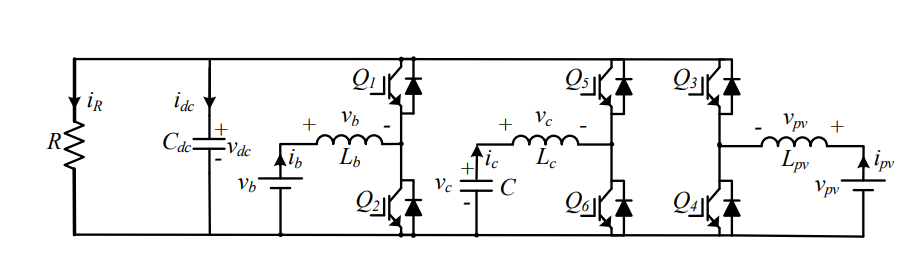
\includegraphics[width=0.5\textwidth]{images/diagrama.png}

    \caption{Diagrama do sistema}
    \label{fig:diagrama}
\end{figure}

Para o chaveamento de cada par de transistores(3 pares), forma implemantados os sinais de PWM, sendo que a condução de um par se comporta de forma complementar entre si, ou seja, quando um transistor está conduzindo, o outro está desligado, tendo ciclos de trabalho de db, dpv e dc, para o par do convesor de bateria de primeira vida, segunda vida e ultracapacitor, respectivamente.

Para o projeto do sistema, deve-se determinar todos os circuitos além dos comportamentos de tensão e corrente sobre LC, e portanto deve projetar os indutores e capacitores para que tenha uma ondulação inverior a 10\% e 20\% da tensaõ em seu respectivo componente para uma determjinada potência.

Após isso, deve-se determinar o modelo de espaço de estados do sistema,validar o sistema com simulações  e então projetar um controlador droop para a malha externa de tensão, com o objetivo de melhorar a resposta do sistema.


Por fim deve-se calcular o comportamento da resposta em frequência da impedância vista pela carga e o comportamento dos autovalores, evidenciando a influência do controle sobre a impedância e sobre a estabilidade.


\subsection{Parâmetros e escopo do projeto}
Foi considerado alguns valores de parâmeteros para o projeto do sistema, indicados pela tabela abaixo:

\begin{table}[H]
    \caption{Parâmetros adotados para o projeto demonstrativo}
    \label{tab:parametros}
    \centering
    \begin{tabular}{llll}
        \toprule
        Grandeza & Valor & Grandeza & Valor \\
        \midrule
        $V_{dc}$                & 400 V          & $V_{c,0}$            & 300 V          \\
        $P_R$                   & 8 kW           &  $V_b$                & 200 V        \\
        $R$                     & 20 $\Omega$    & $V_{pv}$                & 250 V       \\
        $f_s$                   & 20 kHz         & $I_R$                & 20 A           \\
       
        \bottomrule
    \end{tabular}
\end{table}







% Definição do problema
\section{Desenvolvimento}

\subsection{Estados de condução e formas de onda}

Adota-se $v_{dc}>0$, com as correntes $i_b$, $i_c$ e $i_{pv}$ orientadas dos armazenadores para os braços e a corrente $i_R$ orientada do barramento para a carga. Para cada braço $k\in\{b,c,pv\}$, define-se $s_k=1$ quando a chave inferior conduz ($Q_2$, $Q_6$ ou $Q_4$) e $s_k=0$ quando a chave superior conduz ($Q_1$, $Q_5$ ou $Q_3$). Como as chaves de um mesmo braço são complementares, $d_k=\overline{s_k}$ representa a razão cíclica da chave inferior, e $\alpha_k=1-s_k$ define a tensão do ponto médio, $v_{m,k}=\alpha_k v_{dc}$. Aplicando as leis de Kirchhoff, as tensões nos indutores resultam em
\begin{align}
v_{L_b}&=V_b-\alpha_b v_{dc},\nonumber\\
v_{L_c}&=v_c-\alpha_c v_{dc},\label{eq:vL}\\
v_{L_{pv}}&=V_{pv}-\alpha_{pv} v_{dc}.\nonumber
\end{align}
Dessa forma, com a chave inferior ligada o indutor é submetido a $V_k$ e, com a superior ligada, a $V_k-v_{dc}$. Dos $2^3=8$ estados possíveis, nenhum provoca curto-circuito, e todos estão listados na Tabela~\ref{tab:estados}.

\begin{table}[H]
\centering
\caption{Topologias de condução ($s_bs_cs_{pv}$)}
\label{tab:estados}
\footnotesize
\setlength{\tabcolsep}{3pt}
\begin{tabular}{llll}
\toprule
$s_bs_cs_{pv}$ & Chaves ON & Braços no barramento & $C_{dc}\dot v_{dc}$ \\
\midrule
000 & $Q_1,Q_5,Q_3$ & $b,c,pv$ & $i_b+i_c+i_{pv}-i_R$ \\
001 & $Q_1,Q_5,Q_4$ & $b,c$ & $i_b+i_c-i_R$ \\
010 & $Q_1,Q_6,Q_3$ & $b,pv$ & $i_b+i_{pv}-i_R$ \\
011 & $Q_1,Q_6,Q_4$ & $b$ & $i_b-i_R$ \\
100 & $Q_2,Q_5,Q_3$ & $c,pv$ & $i_c+i_{pv}-i_R$ \\
101 & $Q_2,Q_5,Q_4$ & $c$ & $i_c-i_R$ \\
110 & $Q_2,Q_6,Q_3$ & $pv$ & $i_{pv}-i_R$ \\
111 & $Q_2,Q_6,Q_4$ & nenhum & $-i_R$ \\
\bottomrule
\end{tabular}
\end{table}

Em cada intervalo, a derivada da corrente do indutor vale $V_k/L_k$ com a chave inferior ligada e $(V_k-V_{dc})/L_k$ com a superior ligada. Consequentemente, a tensão $v_{L_k}$ é uma onda retangular de dois níveis, a corrente $i_k$ é aproximadamente triangular, a corrente no capacitor do barramento é pulsada e a tensão $v_{dc}$, por ser sua integral, exibe ondulação em dente de serra por partes. A tensão do ultracapacitor, por sua vez, é a integral de $-i_c/C$, decrescendo na descarga e crescendo na recarga. Em regime periódico, impondo valor médio nulo para $v_{L_k}$, obtém-se
\begin{equation}
V_{dc}=\frac{V_b}{1-d_b}=\frac{V_{pv}}{1-d_{pv}}=\frac{V_c}{1-d_c},
\label{eq:ganho}
\end{equation}
sendo a última igualdade apenas quase-estacionária, pois $v_c$ varia ao longo da descarga. A ondulação pico a pico da corrente em cada ramo é dada por
\begin{equation}
\Delta i_{L_k}=\frac{V_k\,d_k}{L_k\,f_s}.
\label{eq:dI}
\end{equation}
A Figura~\ref{fig:ondas} apresenta, para três períodos PWM, os comandos das chaves inferiores, as correntes nos indutores e a tensão do barramento obtidos por simulação.

\begin{figure}[H]
\centering
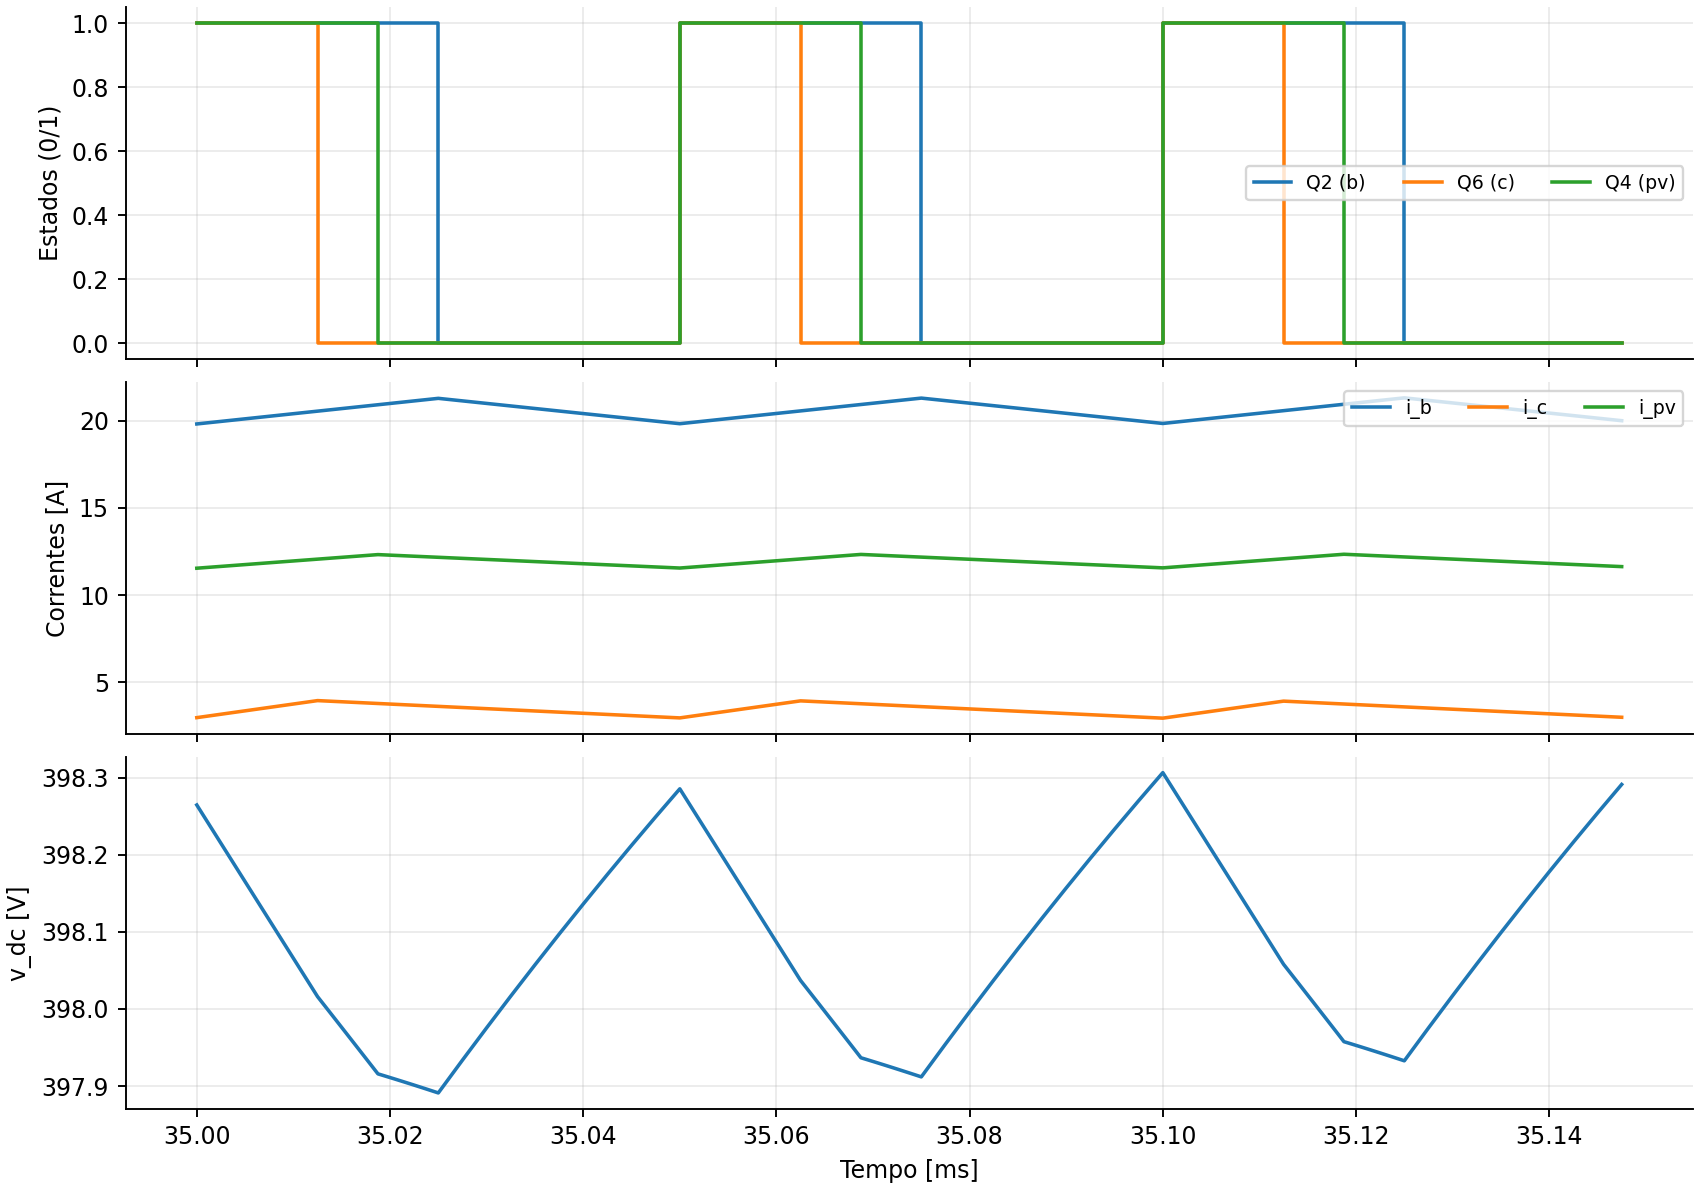
\includegraphics[width=\columnwidth]{images/fig_ondas.png}
\caption{Comandos das chaves inferiores, correntes nos indutores e tensão do barramento em três períodos PWM.}
\label{fig:ondas}
\end{figure}

\subsection{Dimensionamento dos componentes}

No equilíbrio permanente, $i_c=0$ e cada bateria entrega 4 kW, o que resulta em $I_b=20$ A e $I_{pv}=16$ A. Para que os três indutores sejam verificados simultaneamente, considera-se também um modo transitório no qual $P_b=3$ kW, $P_{pv}=2$ kW e $P_c=3$ kW, correspondente a $I_b=15$ A, $I_{pv}=8$ A e $I_c=10$ A. Como a ondulação relativa é maior quanto menor a corrente média, aplica-se \eqref{eq:dI} aos menores valores de corrente, exigindo ondulação de no máximo $10\%$:
\begin{align}
L_b&\ge\frac{200\cdot0{,}5}{0{,}1\cdot15\cdot20000}=3{,}333\ \text{mH},\\
L_{pv}&\ge\frac{250\cdot0{,}375}{0{,}1\cdot8\cdot20000}=5{,}859\ \text{mH},\\
L_c&\ge\frac{300\cdot0{,}25}{0{,}1\cdot10\cdot20000}=3{,}750\ \text{mH}.
\end{align}
Foram adotados valores comerciais ligeiramente superiores, resultando nas ondulações da Tabela~\ref{tab:dim}.

Para o capacitor do barramento, considera-se ondulação máxima de $20\%$, isto é, $\Delta V_{dc,max}=80$ V, e um limite conservador em que a carga descarrega o capacitor durante $d_{max}T_s=0{,}5\,T_s$:
\begin{equation}
C_{dc}\ge\frac{I_R\,d_{max}}{f_s\,\Delta V_{dc,max}}=\frac{20\cdot0{,}5}{20000\cdot80}=6{,}25\ \mu\text{F}.
\end{equation}
Esse limite refere-se apenas à ondulação em regime e não garante bom desempenho em transitórios de potência, razão pela qual se adotou $C_{dc}=1$ mF. Para o ultracapacitor, a capacitância é escolhida por energia e tempo de suporte, e não pela ondulação na frequência de chaveamento. Exigindo que $I_c=10$ A durante 0,5 s provoque $\Delta v_c\le0{,}2\cdot300=60$ V, obtém-se
\begin{equation}
C\ge\frac{I_c\,\Delta t}{\Delta v_c}=\frac{10\cdot0{,}5}{60}=83{,}3\ \text{mF},
\end{equation}
e adotou-se $C=0{,}1$ F, o que resulta em $\Delta v_c=50$ V e em energia liberada de 1375 J entre 300 V e 250 V. Ressalta-se que $d_c$ precisa ser ajustado continuamente à medida que $v_c$ muda, uma vez que a relação estática \eqref{eq:ganho} não pode ser mantida com $d_c$ fixo durante uma descarga prolongada.

\begin{table}[H]
\centering
\caption{Componentes adotados e ondulações obtidas}
\label{tab:dim}
\small
\begin{tabular}{lccc}
\toprule
Componente & Valor mínimo & Adotado & Ondulação \\
\midrule
$L_b$ & 3,333 mH & 3,4 mH & 9,80\% \\
$L_c$ & 3,750 mH & 3,8 mH & 9,87\% \\
$L_{pv}$ & 5,859 mH & 6,0 mH & 9,77\% \\
$C_{dc}$ & 6,25 $\mu$F & 1 mF & 0,08\% \\
$C$ & 83,3 mF & 0,1 F & 16,7\% \\
\bottomrule
\end{tabular}
\end{table}

\subsection{Modelo de espaço de estados}

Escolhendo o vetor de estados $\mathbf{x}=[i_b\ i_c\ i_{pv}\ v_{dc}\ v_c]^\top$, o modelo exato em cada intervalo de condução é
\begin{align}
L_b\dot i_b&=V_b-\alpha_b v_{dc},\nonumber\\
L_c\dot i_c&=v_c-\alpha_c v_{dc},\nonumber\\
L_{pv}\dot i_{pv}&=V_{pv}-\alpha_{pv} v_{dc},\label{eq:chav}\\
C_{dc}\dot v_{dc}&=\alpha_b i_b+\alpha_c i_c+\alpha_{pv} i_{pv}-\frac{v_{dc}}{R},\nonumber\\
C\dot v_c&=-i_c,\nonumber
\end{align}
que pode ser escrito como $\dot{\mathbf{x}}=\mathbf{A}(\alpha)\mathbf{x}+\mathbf{b}$, com as matrizes apresentadas em \eqref{eq:Amat}. Para cada uma das oito configurações da Tabela~\ref{tab:estados}, basta atribuir valores binários a $s_b$, $s_c$ e $s_{pv}$, enquanto o modelo médio em MCC corresponde à mesma expressão com $\alpha_k=1-d_k$.


\begingroup
\footnotesize
\setlength{\arraycolsep}{2.5pt}
\begin{equation}
\mathbf{A}=\begin{bmatrix}
0&0&0&-\dfrac{\alpha_b}{L_b}&0\\[7pt]
0&0&0&-\dfrac{\alpha_c}{L_c}&\dfrac1{L_c}\\[7pt]
0&0&0&-\dfrac{\alpha_{pv}}{L_{pv}}&0\\[7pt]
\dfrac{\alpha_b}{C_{dc}}&\dfrac{\alpha_c}{C_{dc}}&\dfrac{\alpha_{pv}}{C_{dc}}&-\dfrac1{RC_{dc}}&0\\[7pt]
0&-\dfrac1C&0&0&0
\end{bmatrix},\qquad
\mathbf{b}=\begin{bmatrix}\dfrac{V_b}{L_b}\\[7pt]0\\[7pt]\dfrac{V_{pv}}{L_{pv}}\\[7pt]0\\[7pt]0\end{bmatrix}
\label{eq:Amat}
\end{equation}
\begin{equation}
\mathbf{B}_d=\begin{bmatrix}
\dfrac{V_{dc}}{L_b}&0&0\\[7pt]
0&\dfrac{V_{dc}}{L_c}&0\\[7pt]
0&0&\dfrac{V_{dc}}{L_{pv}}\\[7pt]
-\dfrac{I_b}{C_{dc}}&-\dfrac{I_c}{C_{dc}}&-\dfrac{I_{pv}}{C_{dc}}\\[7pt]
0&0&0
\end{bmatrix},\qquad
\mathbf{B}_\ell=\begin{bmatrix}0\\0\\0\\-\dfrac1{C_{dc}}\\0\end{bmatrix}
\label{eq:Bmat}
\end{equation}
\endgroup

Como verificação de consistência, a energia armazenada, $E=\tfrac12\sum_kL_ki_k^2+\tfrac12C_{dc}v_{dc}^2+\tfrac12Cv_c^2$, deve satisfazer
\begin{equation}
\dot E=V_bi_b+V_{pv}i_{pv}-\frac{v_{dc}^2}{R},
\end{equation}
pois o termo $v_ci_c$ se cancela entre $L_c$ e $C$ por tratar-se de uma transferência interna, o que confirma os sinais adotados. Em seguida, linearizando em torno do ponto permanente $(I_b,I_c,I_{pv},V_{dc},V_c)=(20,0,16,400,300)$ com $(d_b,d_c,d_{pv})=(0{,}5,0{,}25,0{,}375)$, obtém-se
\begin{equation}
\dot{\hat{\mathbf{x}}}=\mathbf{A}(d_0)\hat{\mathbf{x}}+\mathbf{B}_d\hat{\mathbf{d}}+\mathbf{B}_\ell\hat i_\ell,
\label{eq:lin}
\end{equation}
com $\mathbf{B}_d$ e $\mathbf{B}_\ell$ dados em \eqref{eq:Bmat}, em que $\hat i_\ell$ é uma corrente incremental adicional extraída do barramento. Cabe destacar que, como $C\dot v_c=-i_c$, um equilíbrio estrito exige $i_c=0$, de modo que uma corrente não nula no ultracapacitor representa necessariamente um processo transitório de descarga ou recarga.

\subsection{Projeto do controlador \textit{droop}}

A estratégia de controle é composta por uma malha interna de corrente em cada indutor e por uma malha externa de tensão com característica de \textit{droop}, tendo sua implementação Figura \ref{fig:blocos}

\begin{figure}[H]
\centering
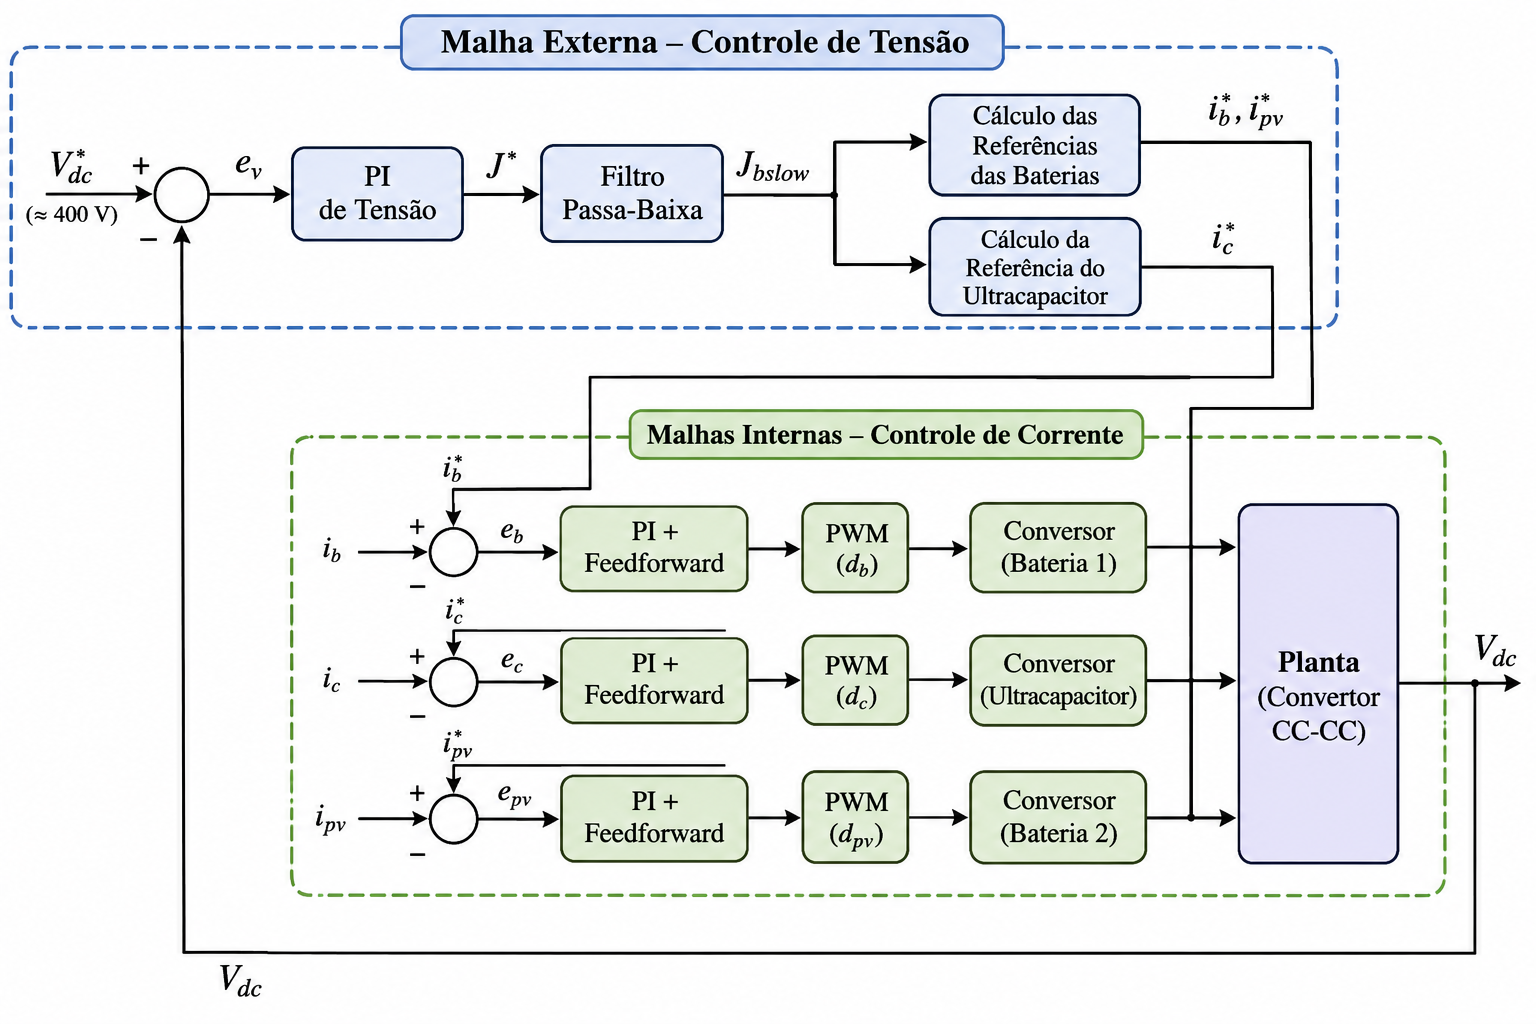
\includegraphics[width=0.9\columnwidth]{images/fig_diagrama_blocos.png}
\caption{Arquitetura do controle em dupla malha.}
\label{fig:blocos}
\end{figure}

Na malha interna, utiliza-se o \textit{feedforward} da tensão de entrada somado a um PI, com saturação das razões cíclicas em $[0{,}02;\,0{,}98]$ e anti-\textit{windup} condicional:
\begin{align}
d_k^{ff}&=1-\frac{V_k}{v_{dc}},\nonumber\\
d_k&=\mathrm{sat}\!\left[d_k^{ff}+K_{pi,k}\,e_k+K_{ii,k}\,\xi_k\right],\label{eq:pi}\\
e_k&=i_k^{\star}-i_k,\qquad\dot\xi_k=e_k.\nonumber
\end{align}
Com o \textit{feedforward} ideal, a planta vista pelo PI reduz-se a $\hat i_k/\hat d_k=V_{dc}/(L_ks)$, de modo que, escolhendo $\omega_{ni}=2\pi\cdot1000$ rad/s e $\zeta=0{,}707$, os ganhos são
\begin{equation}
K_{pi,k}=\frac{2\zeta\omega_{ni}L_k}{V_{dc}},\qquad
K_{ii,k}=\frac{\omega_{ni}^2L_k}{V_{dc}},
\end{equation}
cujos valores constam na Tabela~\ref{tab:ganhos}.

\begin{table}[H]
\centering
\caption{Ganhos da malha interna de corrente}
\label{tab:ganhos}
\small
\begin{tabular}{lcc}
\toprule
Ramo & $K_{pi}$ [A$^{-1}$] & $K_{ii}$ [(A$\cdot$s)$^{-1}$] \\
\midrule
Bateria 1 ($b$) & 0,07552 & 335,567 \\
Ultracapacitor ($c$) & 0,08440 & 375,045 \\
Bateria 2 ($pv$) & 0,13327 & 592,176 \\
\bottomrule
\end{tabular}
\end{table}

Na malha externa, a referência de tensão do barramento decresce com a corrente de carga, caracterizando o \textit{droop}:
\begin{equation}
v_{dc}^{\star}=400-r_d\,(i_R-20),\qquad r_d=1\ \Omega,\qquad i_R=\frac{v_{dc}}{R}.
\end{equation}
Definindo $e_v=v_{dc}^{\star}-v_{dc}$, a corrente total a ser entregue ao barramento é
\begin{equation}
J^{\star}=i_R+K_{pv}\,e_v+K_{iv}\,\xi_v,\qquad\dot\xi_v=e_v.
\end{equation}
Considerando a planta externa simplificada $1/(C_{dc}s+1/R)$, com $\omega_{nv}=2\pi\cdot40$ rad/s e $\zeta=0{,}707$, obtém-se
\begin{align}
K_{pv}&=2\zeta\omega_{nv}C_{dc}-\frac1R=0{,}3054\ \text{A/V},\\
K_{iv}&=\omega_{nv}^2C_{dc}=63{,}17\ \text{A/(V$\cdot$s)}.
\end{align}
Para que o ultracapacitor atenda preferencialmente aos transitórios e as baterias supram a potência média, a demanda é filtrada por $\tau_b\dot J_b^{slow}=J^{\star}-J_b^{slow}$, com $\tau_b=0{,}08$ s. Adotando partilha de $50\%$ entre as baterias, as referências de corrente dos indutores são
\begin{align}
i_b^{\star}&=\frac{0{,}5\,J_b^{slow}}{1-d_b^{ff}},\nonumber\\
i_{pv}^{\star}&=\frac{0{,}5\,J_b^{slow}}{1-d_{pv}^{ff}},\label{eq:refs}\\
i_c^{\star}&=\frac{J^{\star}-J_b^{slow}}{1-d_c^{ff}},\nonumber
\end{align}
em que o fator $1-d_k^{ff}=V_k/v_{dc}$ converte a corrente média desejada no barramento em corrente de indutor. Trata-se de uma escolha de gerenciamento de energia, não da única possível, uma vez que, na prática, exigem-se também limites de temperatura, estado de carga, corrente e potência dos bancos.

% Solução do problema (opcional)
%\section{Desenvolvimento}
\label{Desenvolvimento}
O desenvolvimento teórico apresentado adiante terá como base os livros \cite{nise2015} e \cite{Vilma}, além dos slides disponibilizados pelo docente da disciplina.

\subsection{Descrição de sistemas discretos e sua aplicação em controladores}

Os sistemas discretos são sistemas dinâmicos, cujas variáveis de interesse são definidas em determinados instantes de tempo e em intervalos regulares, como ocorre em dados amostrados em laboratórios. Sendo esse comportamento contrastante com sistemas contínuos, tendo em vista que estes últimos são descritos para qualquer intervalo de tempo.

Na prática, os sistemas discretos são os mais avaliados, tendo em vista que aparelhos de medição, no geral, apresentam limitações físicas; então, os dados coletados por eles são apresentados de forma discreta. Sendo assim, são necessárias ferramentas como a transformada Z para lidar com esses dados.

Além disso, quando se trata de controladores, a análise de sistemas discretos é fundamental, tendo em vista que, na modernidade, a maioria deles é implementada digitalmente. Alguns exemplos que se pode citar dessa prática são: controladores em tempo real com sistemas embarcados, onde sensores obtêm as variáveis do processo, algoritmos computam a ação de controle e os atuadores recebem o sinal processado para a realização da tarefa determinada; além desse exemplo, também é realizado o controle preditivo e adaptativo de sistemas para evitar possíveis falhas em sistemas mais complexos e que, na maioria das vezes, é tratado com o processamento digital de sinais e modelos discretos.

\subsection{Representação de funções discretas}
\label{representacao_frac_parcial}
As funções discretas são aquelas que apresentam valores somente em determinados instantes de tempo, sendo muito comuns em amostragens em laboratórios, ou seja, elas são definidas apenas em instantes de tempo específicos. Em vez de \( x(t) \), que é uma função contínua no tempo, será utilizado, como convenção, \( x[k] \), onde \( k \in \mathbb{Z} \), representando o valor da função no instante de tempo $T_s$\( k \), onde $T_s$ é o período de amostragem e \( k \) o número da amostra, caso \( x[k] \) apresente um número muito elevado de amostras, seu modelo pode, até mesmo, convergir para o valor de \( x(t) \), porém essa convergência em muitos casos não é possível de ser obtida devido a limitações físicas de instrumentos de medição. Essas funções são comuns em sistemas digitais, onde os sinais são amostrados em intervalos regulares, como em processadores digitais de sinais e sistemas de controle discretos.

\subsection{Transformada Z}
Para analisar e projetar sistemas que operam com sinais discretos, utiliza-se a transformada Z, que é uma ferramenta matemática análoga à transformada de Laplace usada em sistemas contínuos. Assim como a transformada de Laplace permite transformar uma função \( x(t) \) do domínio do tempo contínuo para o domínio da frequência complexa \( s \), a transformada Z converte uma sequência discreta \( x[k] \) para o domínio da frequência complexa \( z \).

A transformada Z de uma função \( x[k] \) é definida como:

\begin{equation}
X(z) = \sum_{n=0}^{\infty} x[k] z^{-k},
\label{eq:tz_def}
\end{equation}

Onde \( z \) é a frequência complexa dada por
\begin{equation}
z = r\cdot e^{j\omega},
\label{eq:z_complex}
\end{equation}

Onde \( r \) é a magnitude do número complexo e \( e^{j\omega} \) é a rotação no plano complexo.
Essa transformação facilita a análise de sistemas lineares invariantes no tempo (LTI), permitindo o estudo da estabilidade, resposta em frequência e comportamento dinâmico de sistemas discretos, sendo essas informações de interesse para o desenvolvimento e análise de sistemas e modelos.

Um dos casos mais importantes da transformada Z, tendo em vista que muitos sistemas apresentam esse comportamento, é sua aplicação à função exponencial discreta, definida por:

\begin{equation}
x[n] = a^n u[n],
\label{eq:expo_discreta}
\end{equation}

Onde ‘\( a \)' é uma constante real ou complexa, e \( u[n] \) é a função degrau unitário. A transformada Z dessa função é:

\begin{equation}
X(z) = \sum_{n=0}^{\infty} a^n z^{-n}u[n] = \frac{z}{z - a}, \quad \text{para } |z| > |a|
\label{eq:tz_expo}
\end{equation}




Essa expressão é fundamental, pois muitas outras funções podem ser construídas a partir de combinações de exponenciais, além de representar a resposta de sistemas a entradas exponenciais — o que está diretamente relacionado à análise de polos e estabilidade.

\subsection{Representação em Frações Parciais}

A representação em frações parciais é uma técnica utilizada para decompor funções, que é a razão de polinômios, em uma soma com termos mais simples, ou seja, busca-se transformar uma multiplicação de termos de fração em uma soma. Essa técnica é muito útil na análise de sistemas lineares, tanto no domínio contínuo (com a transformada de Laplace) quanto no domínio discreto (com a transformada Z, que será abordada neste relatório). Tendo como base a função abaixo, que apresenta como polos \( p_1 \) e \( p_2 \), pode-se transformá-la utilizando a expansão em frações parciais em uma soma de frações:

\begin{equation}
Y(t)=\frac{t+1}{(t-p_1)(t-p_2)} = \frac{A}{t-p_1} + \frac{B}{t-p_2},
\label{eq:frac_real}
\end{equation}

Aplicando o limite nos dois termos da equação \ref{eq:frac_real}, tem-se as seguintes igualdades:

\begin{equation}
    \lim_{t \to p_1}\frac{t+1}{(t-p_1)(t-p_2)} (t-p_1)= lim_{t \to p_1} \left(\frac{A}{t-p_1} + \frac{B}{t-p_2}\right) \cdot(t - p_1),
\end{equation}

\begin{equation}
    \lim_{t \to p_2}\frac{t+1}{(t-p_1)(t-p_2)} (t-p_2)= lim_{t \to p_2} \left(\frac{A}{t-p_1} + \frac{B}{t-p_2}\right) \cdot(t - p_2),
\end{equation}

O que resulta em: 

\begin{equation}
\lim_{t \to p_1} Y(t) \cdot (t - p_1) = A,
\label{eq:lim_real_1}
\end{equation}

\begin{equation}
\lim_{t \to p_2} Y(t) \cdot (t - p_2) = B,
\label{eq:lim_real_2}
\end{equation}

Desse modo, pode-se representar frações racionais como soma de frações de polos simples cuja transformada Z é tabelada, demonstrada pela equação \ref{eq:tz_expo}.

Já para funções com polos complexos e conjugados, a obtenção das frações parciais é de forma semelhante, porém trabalhando com números complexos. Além disso, os coeficientes serão conjugados, pois estamos tratando com números reais no sistema e, portanto, a parte imaginária deve se cancelar. Partindo da seguinte função racional:

\begin{equation}
Y(t)=\frac{t+1}{t^2+p_1^2}=\frac{B}{t - jp_1}+\frac{\overline{B}}{t + jp_1},
\label{eq:frac_complex}
\end{equation}

Para esse caso, tem-se que os polos são \( \pm \space jp_1 \).

O cálculo da constante \( B \) é igual a do polo real, isto é, aplicando-se o limite em ambos os lados da equação \ref{eq:frac_complex}, obtendo, desse modo, a seguinte equação:

\begin{equation}
\lim_{t \to jp_1} Y(t)\cdot (t - jp_1) = B,
\label{eq:lim_complex}
\end{equation}

Utilizando essas equações, é possível transformar as funções de transferência no domínio \( z \) para o \( k \) (equivalente de transformar da frequência para o tempo, porém para funções discretas). 

\subsection{Teorema do Valor Final e Inicial}
\label{teorema_valor_in.fin}
\subsubsection{Teorema do Valor Inicial}

Sabe-se que a forma da Transformada Z é dada pela equação \ref{eq:tz_def}.
Fazendo o limite da transformada com \( z \to \infty \), tem-se a seguinte expressão:

\begin{equation}
\lim_{z \to \infty}X(z) = \lim_{z \to \infty}(x[0] + x[1]z^{-1} + x[2]z^{-2} + \ldots),
\label{eq:valor_inicial_exp}
\end{equation}

Para existir o valor inicial, o grau do polinômio do numerador de \( X(z) \) deve ser menor que o do denominador. Caso contrário, o sistema iria divergir para o infinito, aplicando-se o limite descrito na equação \ref{eq:valor_inicial_exp}.

Como \( z^{-n} \to 0 \), quando se aplica o limite presente na equação \ref{eq:valor_inicial_exp}, para \( n \geqslant 1 \). Logo, obtém-se a seguinte relação:

\begin{equation}
x[0] = \lim_{z \to \infty}X(z),
\label{eq:valor_inicial}
\end{equation}

\subsubsection{Teorema do Valor Final}

Além disso, a transformada Z tem a seguinte propriedade:

\begin{equation}
\mathcal{Z}\{x[k+1] - x[k]\} = (z - 1)X(z) - zx[0],
\label{eq:prop_zn_diff}
\end{equation}

Ao olhar para \( x[k+1] - x[k] \), que é a variação entre dois pontos consecutivos da sequência (que tende a 0 em valores muito grandes, no caso de convergência), pode-se reescrever a relação anterior, transportar para o domínio \( Z \), e fazer o limite com \( z \to 1 \), obtendo assim a equação do teorema do valor final:

\begin{equation}
\lim_{k \to \infty} x[k] = \lim_{z \to 1} (1-z^{-1})X(z),
\label{eq:valor_final}
\end{equation}


Para a existência de valor final,os polos devem possuir magnitude menor que 1, ou seja, o valor deve estar dentro do raio unitário, pois como visto na definição da transformada $Z$ na equação \ref{eq:tz_def}, tem-se que se r>1 logo $\lim_{n\to \infty} x[k] \to \infty$ e, portanto, não há convergência nem estabilidade.

\subsection{Estabilidade no domínio ‘z’}
\label{estabilidade}
Para realizar a análise da estabilidade de um sistema descrito no domínio z, deve-se avaliar seus polos. Tendo em vista que os polos dentro do círculo de raio unitário irão contribuir para termos exponenciais decrescentes para uma resposta ao impulso e os polos fora do círculo de raio unitário irão gerar termos exponenciais crescentes. 

Tal comportamento pode ser visualizado através da equação \ref{eq:tz_expo}, na qual a exponencial é representada através de uma série e essa série só irá convergir para valores finitos caso o módulo de ‘a’ seja menor que 1, sendo assim, o sistema só apresentará uma saída que converge caso o polo esteja dentro do círculo unitário.


\subsection{Equação de Bhaskhara:}

A equação de Bhaskhara é uma equação utilizada para encontrar as raízes de um polinômio de segunda ordem, da seguinte forma:

\begin{equation}
    ax^2+bx+c = 0,
\end{equation}

As raízes para esse polinômio serão:

\begin{equation}
    x = \frac{-b \pm \sqrt{b^2-4ac}}{2a},
    \label{bhaskhara}
\end{equation}

Ela é essencial para achar os polos de um sistema com comportamento de segunda ordem e será de extrema importância para achar os polos de um dos sistemas.

% Resultados de implementação
\section{Resultados}

\subsection{Implementação e simulação em Simulink}

A unidade de geração foi implementada em Simulink com solver de passo fixo (\texttt{ode4}) e passo de $T_s/100=0{,}5\ \mu$s, de modo que cada transição de chaveamento seja resolvida com precisão suficiente para a análise das ondulações. O modelo é organizado em quatro blocos: (i) a planta, que implementa as equações \eqref{eq:chav} com os estados $\mathbf{x}$ integrados; (ii) o bloco de PWM, no qual uma portadora dente-de-serra de frequência $f_s$ é comparada com as razões cíclicas, produzindo os sinais $s_b$, $s_c$ e $s_{pv}$; (iii) o controle, que reúne os PI de corrente \eqref{eq:pi}, o \textit{droop}, o filtro de demanda e as referências \eqref{eq:refs}; e (iv) os blocos de aquisição, que registram os estados e as razões cíclicas para o pós-processamento. A carga é uma fonte do tipo degrau, que reduz $R$ de 20~$\Omega$ para 16~$\Omega$ em $t=0{,}1$ s.

Sendo assim, três execuções foram realizadas a partir do mesmo modelo: a primeira com PWM e malha fechada, que fornece os sinais chaveados; a segunda com o modelo médio e malha fechada, em que as razões cíclicas atuam diretamente sobre as equações; e a terceira com razões cíclicas fixas e sem controle, utilizada como referência de comparação. Para os testes de equivalência, o circuito com as chaves $Q_1$ a $Q_6$ foi simulado com os mesmos comandos aplicados às equações, de acordo com a metodologia de três etapas.

\subsection{Verificação da equivalência por simulação em 3 etapas}

Em ambos os casos, a verificação comparou três etapas: o circuito chaveado (etapa 1), as equações chaveadas submetidas aos mesmos sinais PWM (etapa 2) e o modelo médio (etapa 3), este último comparado à média por período do circuito. Como as etapas 2 e 3 recebem apenas as razões cíclicas aplicadas, sem possuir malhas de controle próprias, eventuais diferenças em relação ao circuito decorrem da implementação das equações, das condições iniciais e dos métodos de integração, e não da ação do controlador. O primeiro período de chaveamento foi desconsiderado nas comparações envolvendo o modelo médio, pois a média móvel ainda está se formando.

\textbf{Sem controle.} As razões cíclicas calculadas, $d_b=0{,}5$, $d_c=0{,}25$ e $d_{pv}=0{,}375$, são mantidas constantes, a resistência de carga vale $20~\Omega$ e a simulação parte da condição inicial $\mathbf{x}(0)=(15~\mathrm{A},\,10~\mathrm{A},\,8~\mathrm{A},\,400~\mathrm{V},\,300~\mathrm{V})$. A janela de simulação é de $0{,}45$ s. Como não há regulação da tensão do barramento, $v_{dc}$ apresenta oscilações decorrentes da dinâmica dos indutores e do capacitor $C_{dc}$, enquanto as correntes dos indutores evoluem livremente, sem uma ação de controle que promova sua estabilização. A Figura~\ref{fig:equiv1} apresenta a comparação entre as etapas de simulação, enquanto a Figura~\ref{fig:scope1} apresenta os sinais originais registrados no \textit{Scope}.

\begin{figure}[H]
\centering
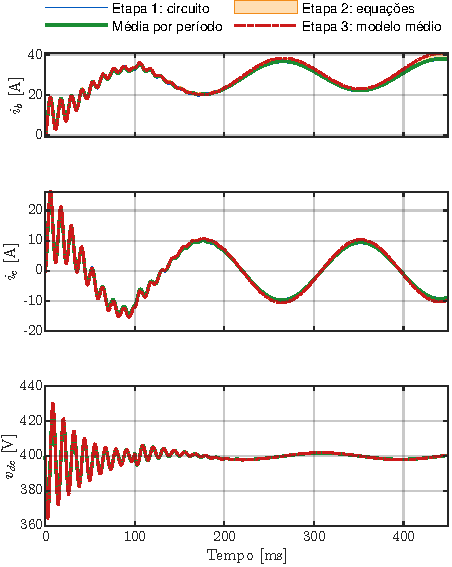
\includegraphics[width=\columnwidth]{images/fig_equiv1.pdf}
\caption{Sem controle: circuito (etapa 1), equações chaveadas (etapa 2), média por período e modelo médio (etapa 3) para $i_b$, $i_c$ e $v_{dc}$.}
\label{fig:equiv1}
\end{figure}

\begin{figure}[H]
\centering
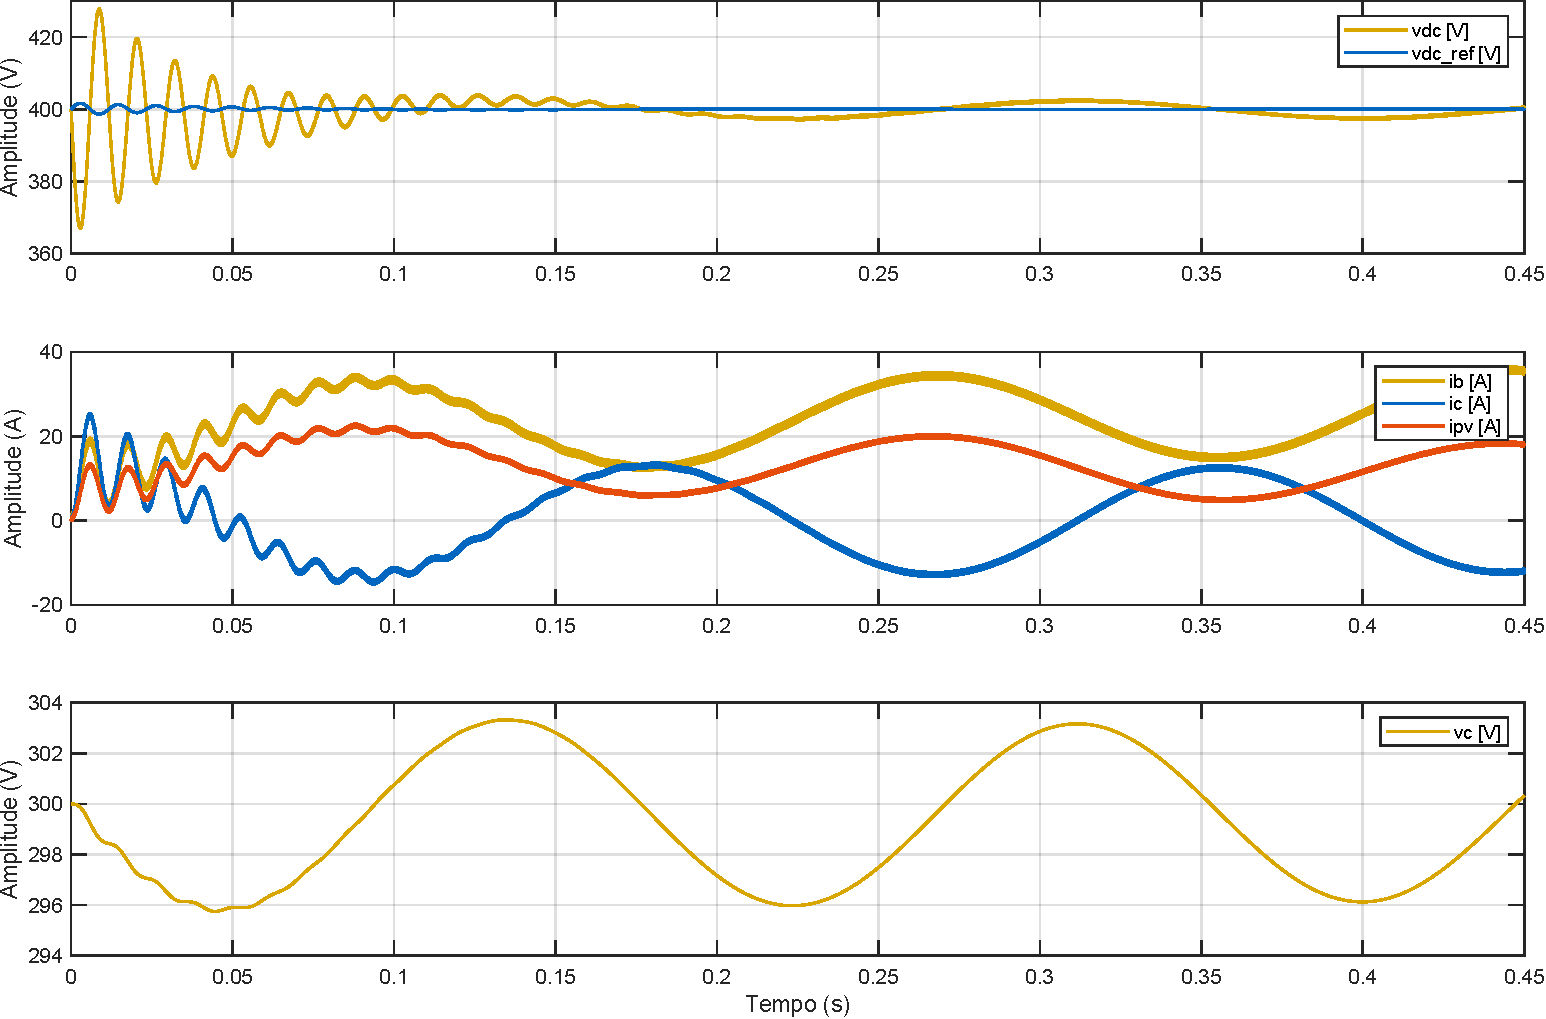
\includegraphics[width=\columnwidth]{images/Dados_semcontrole.pdf}
\caption{Sem controle: sinais do \textit{Scope} ($v_{dc}$, correntes dos indutores e $v_c$).}
\label{fig:scope1}
\end{figure}

 A simulação com controle parte do ponto de equilíbrio $\mathbf{x}(0)=(20~\mathrm{A},\,0~\mathrm{A},\,16~\mathrm{A},\,400~\mathrm{V},\,300~\mathrm{V})$ e, em $t=0{,}1$ s, a resistência de carga passa de $20~\Omega$ para $16~\Omega$. Nesse caso, o degrau provoca um aumento na corrente de carga, dada por $i_R=v_{dc}/R$, e, consequentemente, modifica a referência de tensão do barramento por meio da característica de \textit{droop}:

\begin{equation}
v_{dc}^{\star}=400-r_d(i_R-20),
\end{equation}

que passa de $400$ V para $V_f=395{,}294$ V. Assim, a ação do controlador modifica a dinâmica do sistema e a impedância de saída vista pela carga, ao passo que, no caso sem controle, as razões cíclicas permanecem fixas e não há uma referência de tensão a ser seguida. A Figura~\ref{fig:equiv2} apresenta a comparação entre as etapas de simulação, enquanto a Figura~\ref{fig:scope2} apresenta os sinais registrados no \textit{Scope}, incluindo a tensão do barramento e sua referência.

\begin{figure}[H]
\centering
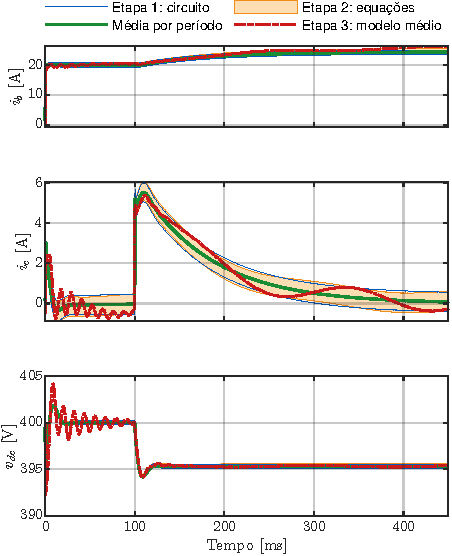
\includegraphics[width=\columnwidth]{images/fig_equiv.pdf}
\caption{Com controle: circuito (etapa 1), equações chaveadas (etapa 2), média por período e modelo médio (etapa 3) para $i_b$, $i_c$ e $v_{dc}$.}
\label{fig:equiv2}
\end{figure}

\begin{figure}[H]
\centering
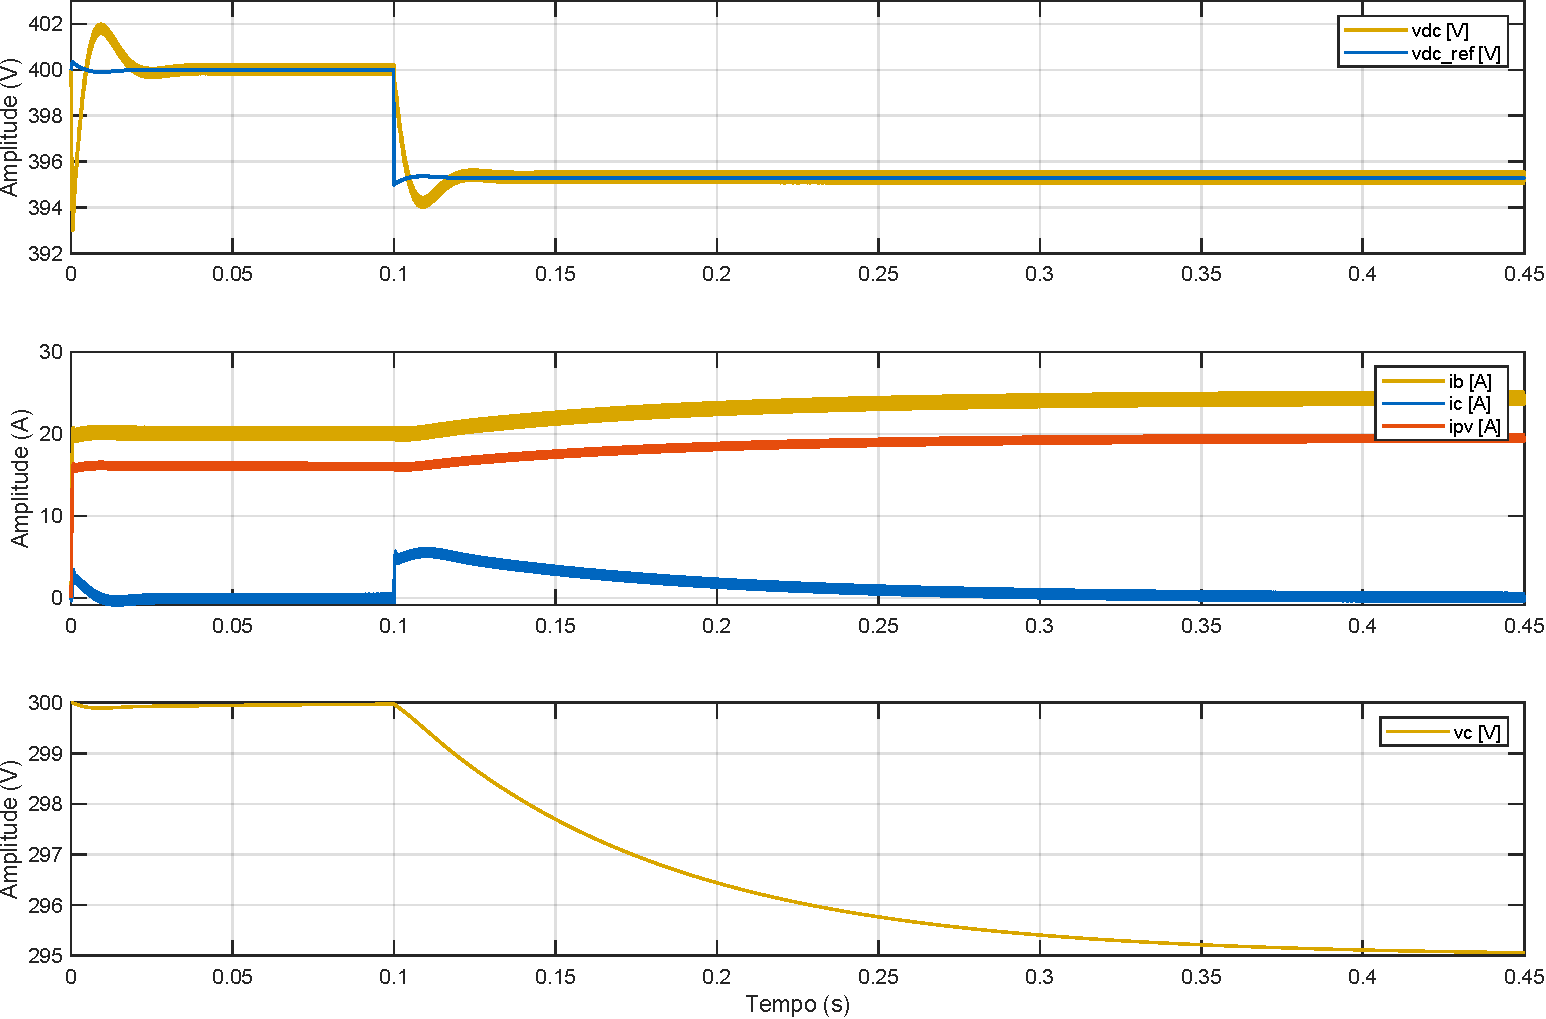
\includegraphics[width=\columnwidth]{Grafico_Conversor.pdf}
\caption{Com controle: sinais do \textit{Scope} ($v_{dc}$, $v_{dc}^{\star}$, correntes dos indutores e $v_c$).}
\label{fig:scope2}
\end{figure}

A Tabela~\ref{tab:erros} quantifica as diferenças entre as etapas 1 e 2 nos dois casos, por meio do erro máximo absoluto e do erro quadrático médio (RMS). A proximidade entre as curvas dessas duas etapas evidencia que as equações chaveadas reproduzem adequadamente o comportamento do circuito, tanto em malha aberta quanto em malha fechada, inclusive durante o degrau de carga.

Na comparação entre a média por período do circuito e o modelo médio, observa-se uma boa correspondência entre as componentes de baixa frequência. As diferenças são decorrentes da aproximação por médias e da frequência PWM finita, uma vez que o modelo médio não reproduz as ondulações de alta frequência associadas ao chaveamento. No caso sem controle, as etapas apresentam comportamentos oscilatórios semelhantes, acompanhando a dinâmica natural do sistema. Já no caso com controle, observa-se a convergência de $v_{dc}$ para a referência imposta pelo \textit{droop}, enquanto a corrente do ultracapacitor atende predominantemente à demanda transitória e retorna gradualmente a zero. Simultaneamente, as baterias aumentam suas contribuições de corrente, assumindo progressivamente o fornecimento de potência em regime permanente. Dessa forma, os resultados confirmam a equivalência entre as representações do sistema e o funcionamento esperado da estratégia de controle.

\begin{table}[H]
\centering
\caption{Erros entre as etapas de simulação, sem e com controle.}
\label{tab:erros}
\footnotesize
\setlength{\tabcolsep}{3pt}
\begin{tabular}{lcccc}
\toprule
& \multicolumn{2}{c}{Sem controle} & \multicolumn{2}{c}{Com controle} \\
\cmidrule(lr){2-3}\cmidrule(lr){4-5}
Grandeza & Máx. 1--2 & RMS média-modelo & Máx. 1--2 & RMS média-modelo \\
\midrule
$i_b$ [A]    & 1,3653 & 1,200 & 0,5385 & 0,927 \\
$i_c$ [A]    & 0,5528 & 0,573 & 0,1149 & 0,388 \\
$i_{pv}$ [A] & 0,8140 & 0,883 & 0,4367 & 0,682 \\
$v_{dc}$ [V] & 0,1258 & 0,476 & 0,0629 & 0,459 \\
$v_c$ [V]    & 0,1469 & 0,153 & 0,0599 & 0,105 \\
\bottomrule
\end{tabular}
\end{table}

\subsection{Impedância, admitância e autovalores}

Tendo em vista que, para uma única resistência fixa, a relação $\hat v_{dc}/\hat i_R=R$ corresponde apenas à lei de Ohm e não à impedância dinâmica de interesse, introduz-se a corrente incremental $\hat i_\ell$ extraída do barramento, conservando-se $R=20\ \Omega$ como carga nominal. Define-se, então,
\begin{align}
G_{vi}(s)&=\frac{\hat v_{dc}(s)}{\hat i_\ell(s)},\\
Z_{out}(s)&=-G_{vi}(s),\\
Y_{out}(s)&=\frac{1}{Z_{out}(s)}.
\end{align}
Linearizando as equações com razões cíclicas fixas e baterias de tensão constante, as correntes incrementais são $\hat i_b=-\alpha_b\hat v_{dc}/(L_bs)$, $\hat i_{pv}=-\alpha_{pv}\hat v_{dc}/(L_{pv}s)$ e $\hat i_c=-\alpha_cs\,\hat v_{dc}/(L_cs^2+1/C)$, de modo que a admitância é
\begin{equation}
Y_{out}(s)=C_{dc}s+\frac1R+\frac{\alpha_b^2}{L_bs}+\frac{\alpha_{pv}^2}{L_{pv}s}+\frac{\alpha_c^2s}{L_cs^2+1/C}.
\label{eq:Y}
\end{equation}
Substituindo $\alpha_b=0{,}5$, $\alpha_c=0{,}75$ e $\alpha_{pv}=0{,}625$, resulta
\begin{equation}
Y_{out}(s)=0{,}001s+0{,}05+\frac{138{,}63}{s}+\frac{0{,}5625\,s}{0{,}0038s^2+10}.
\end{equation}

Para as malhas fechadas, forma-se o vetor aumentado de dez estados $[i_b,\,i_c,\,i_{pv},\,v_{dc},\,v_c,\,\xi_b,\,\xi_c,\,\xi_{pv},\,\xi_v,\,J_b^{slow}]^\top$, cujo jacobiano $\mathbf{A}_{cl}$ é calculado no ponto permanente, e a impedância é obtida por
\begin{equation}
Z_{cl}(s)=-\mathbf{C}_v\,(s\mathbf{I}-\mathbf{A}_{cl})^{-1}\mathbf{B}_\ell,
\end{equation}
em que $\mathbf{C}_v$ seleciona $v_{dc}$. A Figura~\ref{fig:Z} e a Tabela~\ref{tab:Z} comparam as impedâncias com e sem controle. Nota-se que, com razões cíclicas fixas, existem ressonâncias agudas em torno de 6 Hz e de 85 Hz, as quais são amortecidas pelo controle, substituídas por um pico suave próximo de 40 Hz, frequência de projeto da malha de tensão. Acima de algumas centenas de hertz, as duas curvas coincidem, pois a impedância passa a ser dominada pelo capacitor $C_{dc}$.

\begin{figure}[H]
\centering
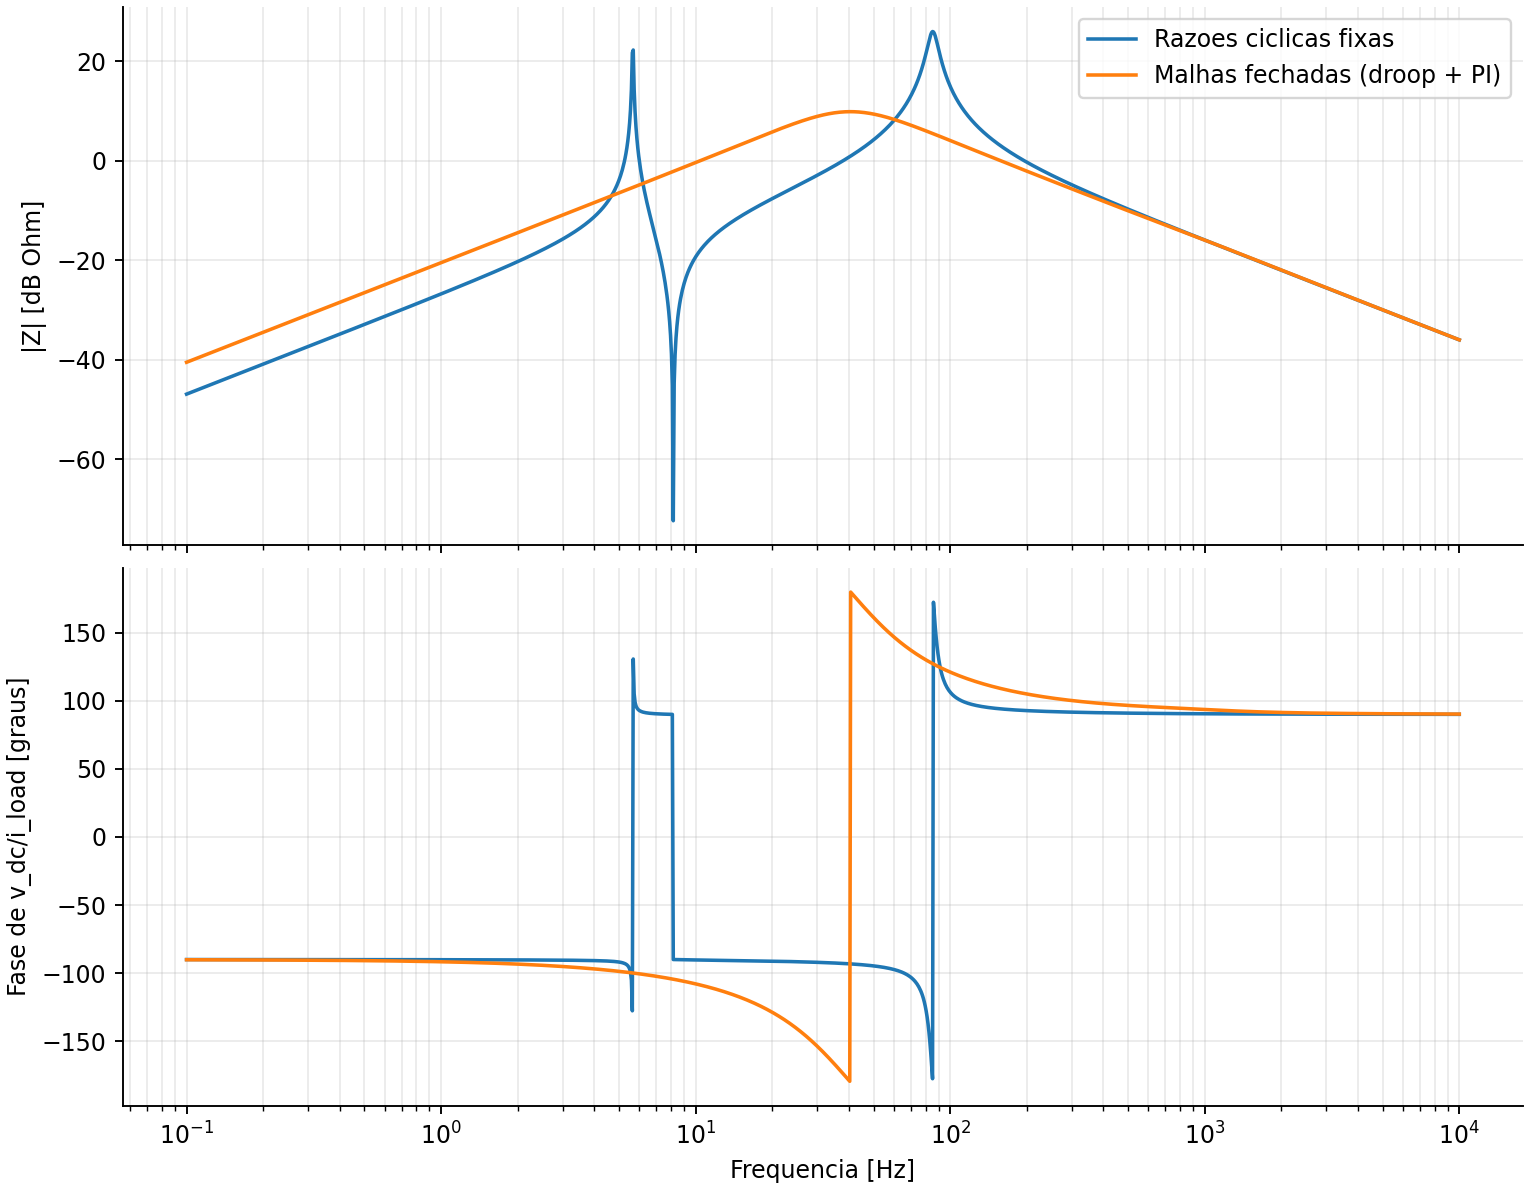
\includegraphics[width=\columnwidth]{images/fig_Z.png}
\caption{Módulo e fase de $Z_{out}$ com razões cíclicas fixas e com PI--\textit{droop}.}
\label{fig:Z}
\end{figure}

\begin{table}[H]
\centering
\caption{$|Z_{out}|$ em malha aberta (razões cíclicas fixas) e em malha fechada}
\label{tab:Z}
\small
\begin{tabular}{rcc}
\toprule
$f$ [Hz] & Razões fixas [$\Omega$] & Controle [$\Omega$] \\
\midrule
1 & 0,0461 & 0,0948 \\
10 & 0,1086 & 0,9639 \\
40 & 1,0914 & 3,1272 \\
100 & 5,6309 & 1,6058 \\
1000 & 0,1603 & 0,1602 \\
\bottomrule
\end{tabular}
\end{table}

Os autovalores do sistema com razões cíclicas fixas são $-24{,}88\pm j536{,}09$, $-0{,}119\pm j35{,}59$ e $0$. Em malha fechada, com os dez estados, obtêm-se $-4415{,}6\pm j4549{,}2$, $-4442{,}2\pm j4443{,}6$ (dois pares), $-157{,}0\pm j200{,}5$, $-12{,}56$ e $0$, apresentados na Figura~\ref{fig:eig}. O autovalor nulo está associado à ausência de regulação explícita do nível de energia do ultracapacitor, pois o controle o utiliza em transitórios sem forçar $v_c$ a um único valor permanente. Os demais modos possuem parte real negativa, e os modos pouco amortecidos da malha aberta, com parte real de $-0{,}119$, passam a ter amortecimento adequado. Contudo, não é correto afirmar estabilidade assintótica de todos os estados sem uma malha adicional de recuperação do estado de carga.

\begin{figure}[H]
\centering
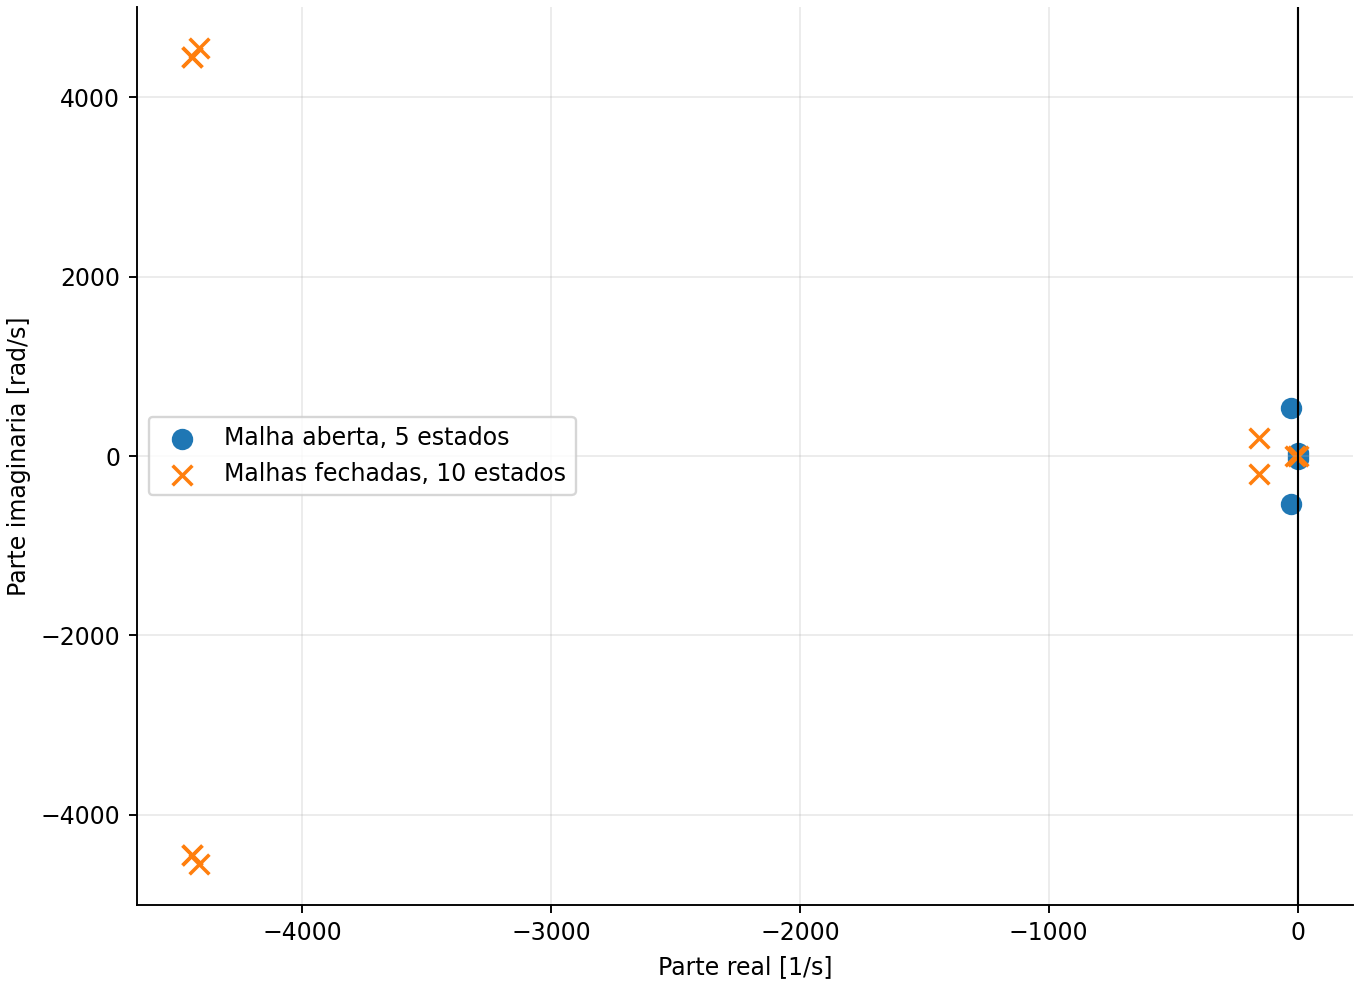
\includegraphics[width=\columnwidth]{images/fig_eig.png}
\caption{Autovalores dos modelos linearizados em malha aberta (5 estados) e fechada (10 estados).}
\label{fig:eig}
\end{figure}


% Análise dos resultados (opcional)
%\input{Capitulos/analise_resultados}

% Conclusões (opcional)
\section{Conclusão}

Foram identificadas as oito configurações de condução do sistema, nas quais cada indutor alterna entre $V_k$ e $V_k-V_{dc}$, gerando corrente aproximadamente triangular. O dimensionamento ($L_b=3{,}4$~mH, $L_{pv}=6$~mH, $L_c=3{,}8$~mH, $C_{dc}=1$~mF, $C=0{,}1$~F) atende às ondulações de 10\% e 20\% adotadas. As equações chaveadas coincidiram com o circuito e o modelo médio reproduziu as componentes de baixa frequência.

O controle em dupla malha (PI de corrente com \textit{feedforward} e \textit{droop} de tensão) fez $v_{dc}$ convergir ao valor previsto de 395,29~V no degrau de carga, com o ultracapacitor atendendo o transitório e as baterias assumindo a demanda lenta. A impedância vista pela carga depende fortemente do controle, que amortece as ressonâncias da malha aberta, e a energia do ultracapacitor precisa de supervisão em longos intervalos, devido ao autovalor nulo.

Os resultados são de simulação ideal (sem perdas, ESR, tempo morto ou amostragem digital), e os valores de projeto são demonstrativos, não dados do enunciado. Uma implementação real exigiria incluir essas não idealidades, limites de corrente e térmicos e gerenciamento de estado de carga.

% ---------- Referências ----------
\printbibliography

% ---------- Anexos (opcional) ----------
%\appendices
%\input{Capitulos/anexos}

\end{document}